% Working BMJ Health \& Care Informatics submission draft; generic review layout, not an official BMJ class.
\documentclass[12pt]{article}
\usepackage[margin=1in]{geometry}

\usepackage{amsmath}
\usepackage{booktabs}
\usepackage{array}
\usepackage{graphicx}
\usepackage{url}

\title{A Reproducibility and Transportability Audit of Cardiovascular Prediction Under Dataset Shift}

\author{Akhil Preetham E, Ch Hari Krishna, G Vennela\par Department of Computer Science and Engineering\par Prasad V. Potluri Siddhartha Institute of Technology, Vijayawada, India\par\small Author order and affiliation are provisional and require confirmation by all authors.}
\begin{document}
\maketitle

\begin{abstract}
This work audits whether a leakage-controlled, multi-source cardiovascular
prediction workflow transports to datasets outside its training sources. On the
separately reported, endpoint-aligned AngioCAD site cohort, the primary
source-only analysis achieved
ROC-AUC 0.787 (95\% conditional interval 0.734--0.838), while calibrated
10-bin expected calibration error was 0.216 and feature-only out-of-distribution
AUROC was 0.589 (0.541--0.635). AngioCAD reported 413 labeled IDs, but only 377
had matching feature rows; the public workbook does not document age or fasting
blood-sugar units. Cross-dataset patient independence is unverified, and
AngioCAD labels had been inspected before subsequent reliability analyses. In
a post-hoc replay, the integrated selective rule emitted
21/377 outputs (5.6\%), all for positive cases, which is too small and
one-class to establish useful risk control. A metadata-based site gate
withheld scores for every unregistered site. Duke supplied a separate stress
test with a different stenosis threshold. The evidence supports a reproducible
engineering audit with negative transportability findings; it does not
establish dependable calibration, useful unseen-site coverage, or feature-only
shift recognition.
\end{abstract}

\noindent\textbf{Keywords:} cardiovascular disease; leakage control; nested validation; explainable AI; calibration; conformal prediction; selective prediction; dataset shift; transportability.

\section{Introduction}
Cardiovascular prediction models must be evaluated for discrimination,
calibration, robustness, and transportability rather than accuracy alone.
CARDIODIAG provides an important starting point because it combines explainable
feature reduction with optimized ensemble classifiers \cite{khan2026cardiodiag}.
The active question is whether a model trained across source cohorts can
preserve useful discrimination and probability reliability on unseen sites,
and whether its inference policy can withhold scores outside its registered
operating domain. The broader stability audit remains a complementary
question. Selective reliability is measured empirically and is not treated as
evidence that a model semantically understands uncertainty.

\textbf{Contribution status.} The supported contribution is a reproducible
engineering evaluation of multi-source transfer, source-only uncertainty and
calibration, feature-only shift diagnostics, and a fail-closed unknown-site
policy, supplemented by a stability--reliability decoupling analysis. The
evidence includes a negative result: stable feature selection did not yield a
consistent reliability advantage, and feature-only shift detection was weak on
  the aligned external site. No new prediction algorithm is claimed. The available
  records do not establish patient-level independence across sites; one site does
  not establish broad generalization or clinical utility.

\section{Related Work and Research Gap}
Feature-selection stability is an established property of a selection procedure,
not a substitute for predictive validation. Nogueira \emph{et al.} provide a
chance-corrected stability statistic for comparing selected sets
\cite{nogueira2018stability}, while resampling-based stability selection has
distinct assumptions and error-control goals \cite{meinshausen2010stability}.
Nested validation is required when the same data support model selection and
performance estimation \cite{varma2006bias,cawley2010overfitting}. Calibration,
discrimination, and selective risk are likewise distinct properties of a
prediction model \cite{vancalster2019calibration}. Conformal prediction can
provide marginal coverage under exchangeability, but coverage should not be
assumed under population shift \cite{angelopoulos2023conformal}.

The research question is whether training-only feature-set stability in the
CARDIODIAG representation is associated with held-out predictive and selective
reliability, and whether source-only uncertainty methods remain informative
under dataset shift. This is an evaluation question, not a claim that the
combination is unprecedented. The reporting and risk-of-bias framing follows
TRIPOD+AI and PROBAST+AI
\cite{collins2024tripodai,moons2025probastai}.

\section{Audit of the Original Implementation}
The supplied repository is notebook-centric and contains multiple historical
protocols. The historical reproduction and its deviations are documented in
\texttt{docs/baseline\_reproduction\_report.md}. In particular, available
notebooks contain paths where resampling, preprocessing, and dimensionality
reduction occur before the evaluation split.

\subsection{Historical Reproduction Claims}
The original paper's reported protocol cannot be reproduced bit-for-bit from
the supplied notebooks: split sizes, preprocessing order, model blocks, search
grids, and saved tables are inconsistent. The native reproduction path
specified in the audit applied SMOTE before an 80/20 split without
stratification; on \texttt{heart5.csv} it produced 1,016 rows after SMOTE and
reported OSEC accuracy 0.8873, ROC-AUC 0.9516, and Brier score 0.0890, while
OVEC reported accuracy 0.8627, ROC-AUC 0.9163, and Brier score 0.1236. These
are protocol-specific reproduction artifacts, not leakage-controlled
generalization estimates. The corrected single-split comparison reported
OSEC accuracy 0.8957, ROC-AUC 0.9348, and Brier score 0.0875, with stable OSEC
accuracy 0.9000, ROC-AUC 0.9360, and Brier score 0.0864; these values are
not the primary corrected evidence because they use one split. Accordingly,
the original paper's numerical claims are not treated as validated
corrected-pipeline results.

\section{Methods}
\subsection{Corrected Pipeline}
All data-dependent operations are fitted on the training data of the relevant
fold. Feature types are declared in the local dataset manifest: nominal and
ordinal coded predictors are one-hot encoded, identifiers are excluded, and
numeric missingness/outlier treatment is training-only. Unknown external data
must provide an explicit feature mapping before the external gate can pass.
The boundary flow is summarized in Fig.~\ref{fig:workflow}.

\begin{figure*}[t]
\centering
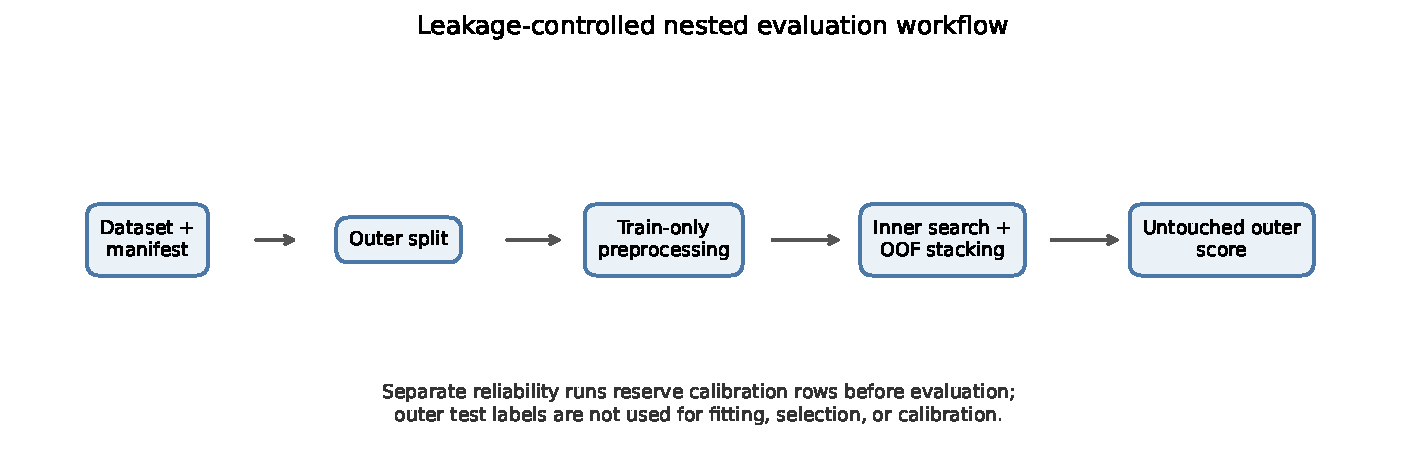
\includegraphics[width=0.98\textwidth]{figures/master_directive_20261105_final/research_workflow.pdf}
\caption{Leakage-controlled nested evaluation. Preprocessing, model selection,
and out-of-fold stacking are confined to the outer training partition; the
outer test fold is scored once. Separate reliability experiments reserve
calibration data before evaluation.}
\label{fig:workflow}
\end{figure*}

\subsection{Stability-Aware Feature Reduction}
For feature $j$ and inner resample $b$, let $r_{j,b}$ denote the combined
training-only relevance score and $s_{j,b}$ its selection indicator. Relevance
is estimated after splitting each resample into a fitting part and a validation
part; permutation importance is evaluated on the latter, which remains inside
the outer training boundary. We define
\begin{equation}
\pi_j = \frac{1}{B}\sum_{b=1}^{B}s_{j,b}, \qquad
\bar r_j = \frac{1}{B}\sum_{b=1}^{B}r_{j,b}.
\end{equation}
Features are retained when their selection frequency and mean relevance pass
the prespecified thresholds. To test whether this improves stability, the
selected sets are compared with a single-pass relevance selector over matched
repeated stratified training perturbations using the chance-corrected stability
statistic of Nogueira \emph{et al.} \cite{nogueira2018stability}. The reported
interval is a paired bootstrap interval over repeat-level stability estimates.
This is an operational stability rule, not a causal interpretation of feature
importance.

\subsection{Uncertainty and Calibration}
The project reports Brier score, reliability-bin error, calibration intercept
and slope, split-conformal prediction-set coverage, abstention rate, confidence-
error AUC, area under the risk-coverage curve (AURC), and selective risk. The
confidence-error AUC tests whether confidence ranks correct predictions above
errors; it is not a probability of correctness. Conformal coverage is
interpreted under its exchangeability assumption \cite{angelopoulos2023conformal}
and is measured again under any available dataset shift.
The implementation uses ten uniform bins for ECE, omits empty bins, and
averages the remaining absolute calibration gaps equally. Its AURC value is
the arithmetic mean of cumulative error risks over retained-prefix sizes,
rather than a numerically integrated curve; this implementation detail limits
direct comparison with studies using a different AURC convention.

\section{Experimental Protocol}
The historical protocol, corrected common-split protocol, and nested-validation
protocol are kept separate. Hyperparameter selection is performed only in inner
folds. The final internal holdout is not repeatedly consulted. Reporting follows
the transparency principles of TRIPOD+AI \cite{collins2024tripodai} and the
development/evaluation distinctions in PROBAST+AI \cite{moons2025probastai}.

For feature-selection stability, five stratified folds were repeated three
times. The stable selector was compared with a one-shot selector using the
recorded training-fold feature selections. The standalone corrected stability artifacts used eight relevance resamples,
whereas the stable selector embedded in the nested and linkage pipelines used
six. For selective reliability and the paired stability--reliability analysis,
ten random seeds (42--51) used a 56.25\%
fitting, 18.75\% calibration, and 25\% evaluation split. Evaluation labels were
not used for fitting or calibration. These bounded repeated analyses are
exploratory and are not substitutes for a full confirmatory evaluation.

The primary nested endpoint is outer-fold ROC-AUC for the listed candidates;
the stability--reliability linkage is an exploratory paired comparison of
stable OSEC against corrected OSEC. PR-AUC, Brier score, calibration,
feature stability, and selective metrics are secondary. The reported intervals
are descriptive bootstrap summaries over the recorded folds, repeat-level
stability summaries, or seeds; they are not independent-patient confidence
intervals.

As a separate exploratory benchmark, the 70,000-row Kaggle \texttt{cardio}
task was evaluated with three shared stratified outer folds, two inner folds,
seed 42, and bounded inner searches for Logistic regression, Random Forest,
HistGradientBoosting, XGBoost, LightGBM, and CatBoost. This task has a
different target and schema and is not pooled with the two CARDIODIAG
benchmarks. A fixed one-third out-of-fold ensemble of XGBoost,
HistGradientBoosting, and Logistic regression was evaluated on the same outer
folds.

\subsection{Multi-source Shift Evaluation}
The multi-source experiments used Cleveland, Hungary, Switzerland, and VA Long
Beach as training domains. CD-XD-002 used the 13 shared UCI predictors for
retrospective leave-one-source-out evaluation. CD-XD-003 and CD-XD-004 used
age, sex, and fasting-glucose status with a 20\% source-only calibration
partition. For the subsequent reliability-layer experiments CD-XD-005
(Duke) and CD-XD-006 (AngioCAD), each source cohort was stratified into
disjoint partitions: 70\% model fitting, 15\% Platt probability calibration,
and 15\% conformal/OOD threshold calibration. Logistic regression used equal
total fit weight per cohort; Platt calibration used equal total weight per
cohort. Preprocessing and imputers were fit only on model-fitting rows.

The reliability layer formed binary split-conformal sets from calibrated
nonconformity scores \(1-p(y)\), using the maximum of the per-source
finite-sample 90\% quantiles. The feature-support score was mean Euclidean
distance to the 10 nearest source-fitting rows, with a per-source 95\%
calibration threshold. Isolation Forest was retained as an OOD comparator. An
inference bundle returned a prediction and probability only for a registered
source-domain identifier when the conformal set was singleton and the
feature-support score was within threshold. All abstentions withheld the
probability, and out-of-support rows also withheld the conformal set; a new or
missing domain identifier caused abstention before scoring. The identifier is
trusted provenance metadata, not inferred by the model. External labels were
used only for scoring. The AngioCAD reliability replay is post hoc because its target had
already been examined in CD-XD-004. Target bootstrap intervals use 1,000
class-stratified resamples and condition on observed class counts.

\section{Datasets and Provenance}
The 918-row Five States file is a derived composite used as a historical
development benchmark. A row-level audit maps all 918 rows to observed fields
and labels in the UCI Heart Disease components (914 unique matches and four
ambiguous matches due to source missingness). However, the exact upstream
1,190-row Kaggle artifact, its version, license, and complete transformation
and imputation history were not recovered. The Five States file therefore has
unresolved standalone licensing and is not independent of its UCI components.
The UCI Heart Disease record is CC BY 4.0 \cite{ucihd}, but that license alone
does not clear the whole derived composite for redistribution. The Mendeley
Cardiovascular Disease Dataset, version 1, is attributed to Doppala and
Bhattacharyya~\cite{doppala2021dataset} (DOI:
\url{https://doi.org/10.17632/dzz48mvjht.1}) and declares CC BY 4.0. It was
used by the base study and is retained as historical benchmark replication;
the codebook provides no diagnostic reference standard, angiographic
threshold, or predictor index time. Neither benchmark establishes prospective
pre-diagnostic performance.

The four UCI Heart Disease cohorts (Cleveland, Hungary, Switzerland, and VA
Long Beach; 920 records total; DOI \texttt{10.24432/C52P4X}) were used in the
retrospective CD-XD-002 leave-one-source-out pilot. These component records
overlap the Five States composite. The UCI Statlog (Heart) release (270 rows;
DOI \texttt{10.24432/C57303}) was screened but excluded as a new cohort: all
270 rows exactly match Cleveland after binary-label harmonization
\cite{ucistatlog}. These experiments
are retrospective source-domain stress tests and are not independent external
validation.

The UCI Z-Alizadeh Sani cohort contains 303 patients from the reported Shahid
Rajaei center in Tehran~\cite{alizadehsani2013cad,uciz}. It was used in
CD-XD-003 as a transport stress test using age, sex, and fasting-glucose
status. Its CAD target uses \(\geq50\%\) stenosis versus the source
\(>50\%\) definition; the public workbook has no person identifiers for
cross-source linkage. This source was already examined and is not a pristine
confirmatory test.

AngioCAD reports 413 labelled IDs from Shahid Chamran Heart Center in Isfahan
\cite{angiocad2026,angiocadzenodo2025}; only 377 have matching clinical
feature rows. CD-XD-004 derives a target above 50\% from 15 artery-segment
labels and uses age, sex, and binary fasting-glucose status. The release's
negative 26--50\% bin prevents isolating exact-50\% cases. The workbook does
not document age or FBS units, so the historical age-as-years and FBS-as-mg/dL
mappings are assumptions; the post-hoc FBS-excluded replay retains a
provisional age mapping. The 36 unmatched IDs are not imputed, and the reason
for their absence is unknown. AngioCAD is a separately reported site cohort,
but common person identifiers are unavailable; participant-level
independence from source cohorts is unverified. Its outcomes were examined in
CD-XD-004 before subsequent reliability analyses, so it is not an untouched
final test.

The 2026 Mendeley Heart Disease Clinical release (version 1, DOI
\texttt{10.17632/nt4y898vyh.1}, CC BY 4.0) was used only for provenance
screening~\cite{mendeleyheart2026};
all 918 labelled rows exactly match Five States. The 70,000-row Kaggle
Cardiovascular Disease benchmark has a different examination-time target and
schema, and Kaggle lists its license as \texttt{Unknown}~\cite{kagglecardio70k}; it is neither an external
CAD validation set nor cleared for redistribution. Duke ACATH contains 3,504
patients from the Duke Cardiovascular Disease Databank, distributed by
Vanderbilt Biostatistics~\cite{dukeacath2026}. The provider permits use with
attribution, but does not specify standardized redistribution rights. Its
\texttt{>=75\%} stenosis endpoint differs from UCI's \texttt{>50\%}, and
cholesterol is missing in 1,246 records. CD-XD-005 is therefore an
exploratory, endpoint-mismatched stress test, not independent same-endpoint
validation.

No ECG waveform, heart-failure mortality, or post-MI complication dataset was
merged into this tabular CAD task. Those datasets have different modalities,
populations, outcome definitions, or prediction times and would require
separate protocols. Dataset DOIs, versions, hashes, access terms and
attribution notices are recorded in the final dataset attribution register
and dataset-specific notices.

The public Mendeley codebook defines only binary disease presence or absence;
the diagnostic reference standard and threshold are unspecified. It lists
demographics, symptoms, laboratory, ECG, and exercise-test fields, but gives no
collection time or intended prediction point for any predictor. The source
article maps \texttt{noofmajorvessels} to the number of major vessels seen by
fluoroscopy~\cite{doppala2022ensemble}; this is a possible outcome proxy, and
its timing is unknown. The identifier \texttt{patientid} is excluded. The
remaining variables cannot be established as pre-diagnostic from this
release, so Mendeley results are retrospective benchmark replication only.
A same-split feature-exclusion sensitivity is reported in
Section~\ref{sec:validity-sensitivity}.

\begin{table*}[t]
\centering
\caption{Mendeley codebook and predictor-timing audit. No predictor has a
documented measurement time relative to the target. The dataset is retained as
a retrospective benchmark, not a pre-diagnostic cohort.}
\label{tab:mendeley-provenance}
\scriptsize
\setlength{\tabcolsep}{3pt}
\begin{tabular}{@{}>{\raggedright\arraybackslash}p{2.0cm}>{\raggedright\arraybackslash}p{4.8cm}>{\raggedright\arraybackslash}p{6.1cm}>{\raggedright\arraybackslash}p{2.9cm}@{}}
\toprule
Field & Codebook meaning & Provenance / timing assessment & Disposition \\
\midrule
\texttt{patient\allowbreak id} & Patient identification number & Administrative identifier; possible row/source encoding & Exclude \\
\texttt{age} & Age in years & Demographic; collection time and availability at prediction are absent & Retrospective benchmark only \\
\texttt{gender} & 0 female, 1 male & Demographic; collection time absent & Retrospective benchmark only \\
\texttt{chest\allowbreak pain} & Typical, atypical, non-anginal, asymptomatic & Symptom; relation to diagnosis and index time unknown & Timing unclear \\
\texttt{restingBP} & Resting blood pressure, mmHg & Setting, treatment state, and measurement time unknown & Timing unclear \\
\texttt{serum\allowbreak cholestrol} & Serum cholesterol, mg/dL & Sample timing, fasting status, and treatment unknown & Timing unclear \\
\texttt{fasting\allowbreak blood\allowbreak sugar} & Binary indicator for >120 mg/dL & Measurement time and testing protocol unknown & Timing unclear \\
\texttt{resting\allowbreak relectro} & Normal, ST--T abnormality, or probable/definite LVH & ECG-derived diagnostic evidence; timing unknown & Potential outcome-proximal field \\
\texttt{max\allowbreak heartrate} & Maximum heart rate achieved & Test context and timing not given & Potentially test-derived; timing unclear \\
\texttt{exercise\allowbreak angia} & Exercise-induced angina, 0/1 & Exercise-test protocol and timing unknown & Potentially test-derived \\
\texttt{oldpeak} & Numeric ST-related field, range 0--6.2 & Measurement protocol and timing unknown & Potential outcome-proximal field \\
\texttt{slope} & Peak-exercise ST slope category & Exercise-test-derived; time relative to target unknown & Potentially post-diagnostic \\
\texttt{noof\allowbreak major\allowbreak vessels} & 0--3; count seen by fluoroscopy & Angiographic evidence can be downstream of diagnosis & Possible outcome proxy; timing unknown \\
\texttt{target} & 0 absence / 1 presence of heart disease & No reference standard, stenosis threshold, adjudication, or index date supplied & Do not equate to UCI/AngioCAD endpoint \\
\bottomrule
\end{tabular}
\end{table*}

The Duke ACATH cohort contains 3,504 patients referred for chest pain and is
provided by the Vanderbilt Department of Biostatistics from the Duke
Cardiovascular Disease Databank \cite{dukeacath2026}. Its \texttt{sigdz}
endpoint is significant disease at \(\geq 75\%\) diameter narrowing, compared
with \(>50\%\) in the UCI source. CD-XD-005 used age, sex, and serum
cholesterol; cholesterol was missing for 1,246 patients. Duke sex coding was
mapped to the UCI convention. This separately reported site supplies an
endpoint-mismatched transport stress test; person-level independence from
development data is unverified.

The UCI Statlog (Heart) release was screened as a possible additional cohort.
After harmonizing its binary label to the UCI \texttt{num>0} convention, all 270
Statlog records exactly matched Cleveland on the 13 predictors and outcome;
it was therefore excluded as a new cohort rather than counted as a fifth
source; the source record is available at
\url{https://archive.ics.uci.edu/dataset/145/statlog+heart}.

\section{Results}
Table~\ref{tab:nested} reports the post-boundary-corrected nested-validation
artifacts. It is internal evidence only and must not be described as
independent external evidence. Earlier historical and schema-corrected
artifacts remain available under their original prefixes and are not silently
replaced.

\begin{table*}[t]
\centering
\caption{Nested internal validation summary.}
\label{tab:nested}
\begin{tabular}{llrrrrr}
\toprule
Dataset & Candidate & ROC-AUC & PR-AUC & Brier & ECE & ROC-AUC CI \\
\midrule
heart5.csv & corrected\_logistic & 0.928 $\pm$ 0.006 & 0.935 & 0.107 & 0.102 & [0.907, 0.942] \\
heart5.csv & corrected\_ovec & 0.930 $\pm$ 0.007 & 0.933 & 0.100 & 0.086 & [0.909, 0.944] \\
heart5.csv & corrected\_osec & 0.926 $\pm$ 0.011 & 0.928 & 0.112 & 0.121 & [0.889, 0.930] \\
heart5.csv & stable\_logistic & 0.928 $\pm$ 0.006 & 0.935 & 0.107 & 0.109 & [0.907, 0.942] \\
heart5.csv & stable\_osec & 0.925 $\pm$ 0.010 & 0.929 & 0.109 & 0.113 & [0.896, 0.934] \\
MendeleyCardiovascular\_Disease\_Dataset.csv & corrected\_logistic & 0.993 $\pm$ 0.004 & 0.994 & 0.027 & 0.152 & [0.988, 0.996] \\
MendeleyCardiovascular\_Disease\_Dataset.csv & corrected\_ovec & 0.996 $\pm$ 0.001 & 0.997 & 0.025 & 0.158 & [0.992, 0.998] \\
MendeleyCardiovascular\_Disease\_Dataset.csv & corrected\_osec & 0.994 $\pm$ 0.004 & 0.995 & 0.023 & 0.200 & [0.986, 0.997] \\
MendeleyCardiovascular\_Disease\_Dataset.csv & stable\_logistic & 0.993 $\pm$ 0.004 & 0.994 & 0.027 & 0.140 & [0.988, 0.996] \\
MendeleyCardiovascular\_Disease\_Dataset.csv & stable\_osec & 0.994 $\pm$ 0.004 & 0.995 & 0.023 & 0.242 & [0.986, 0.997] \\
\bottomrule
\end{tabular}

\end{table*}

Figure~\ref{fig:nested-curves} visualizes pooled outer-fold predictions; its
pooled curve scores are distinct from the fold-mean metrics in
Table~\ref{tab:nested}. Figures~\ref{fig:calibration} and
\ref{fig:risk-coverage} show complementary probability and abstention
diagnostics. Figure~\ref{fig:confusion} shows fixed-threshold error counts;
Fig.~\ref{fig:feature-stability} summarizes feature selection frequency,
Fig.~\ref{fig:distribution-shift} shows unlabelled distribution differences,
Fig.~\ref{fig:aura-ablation} reports exploratory AURA-ML ablations, and
Fig.~\ref{fig:stress-tests} shows synthetic stress tests. None supplies
independent validation.

\begin{figure*}[t]
\centering
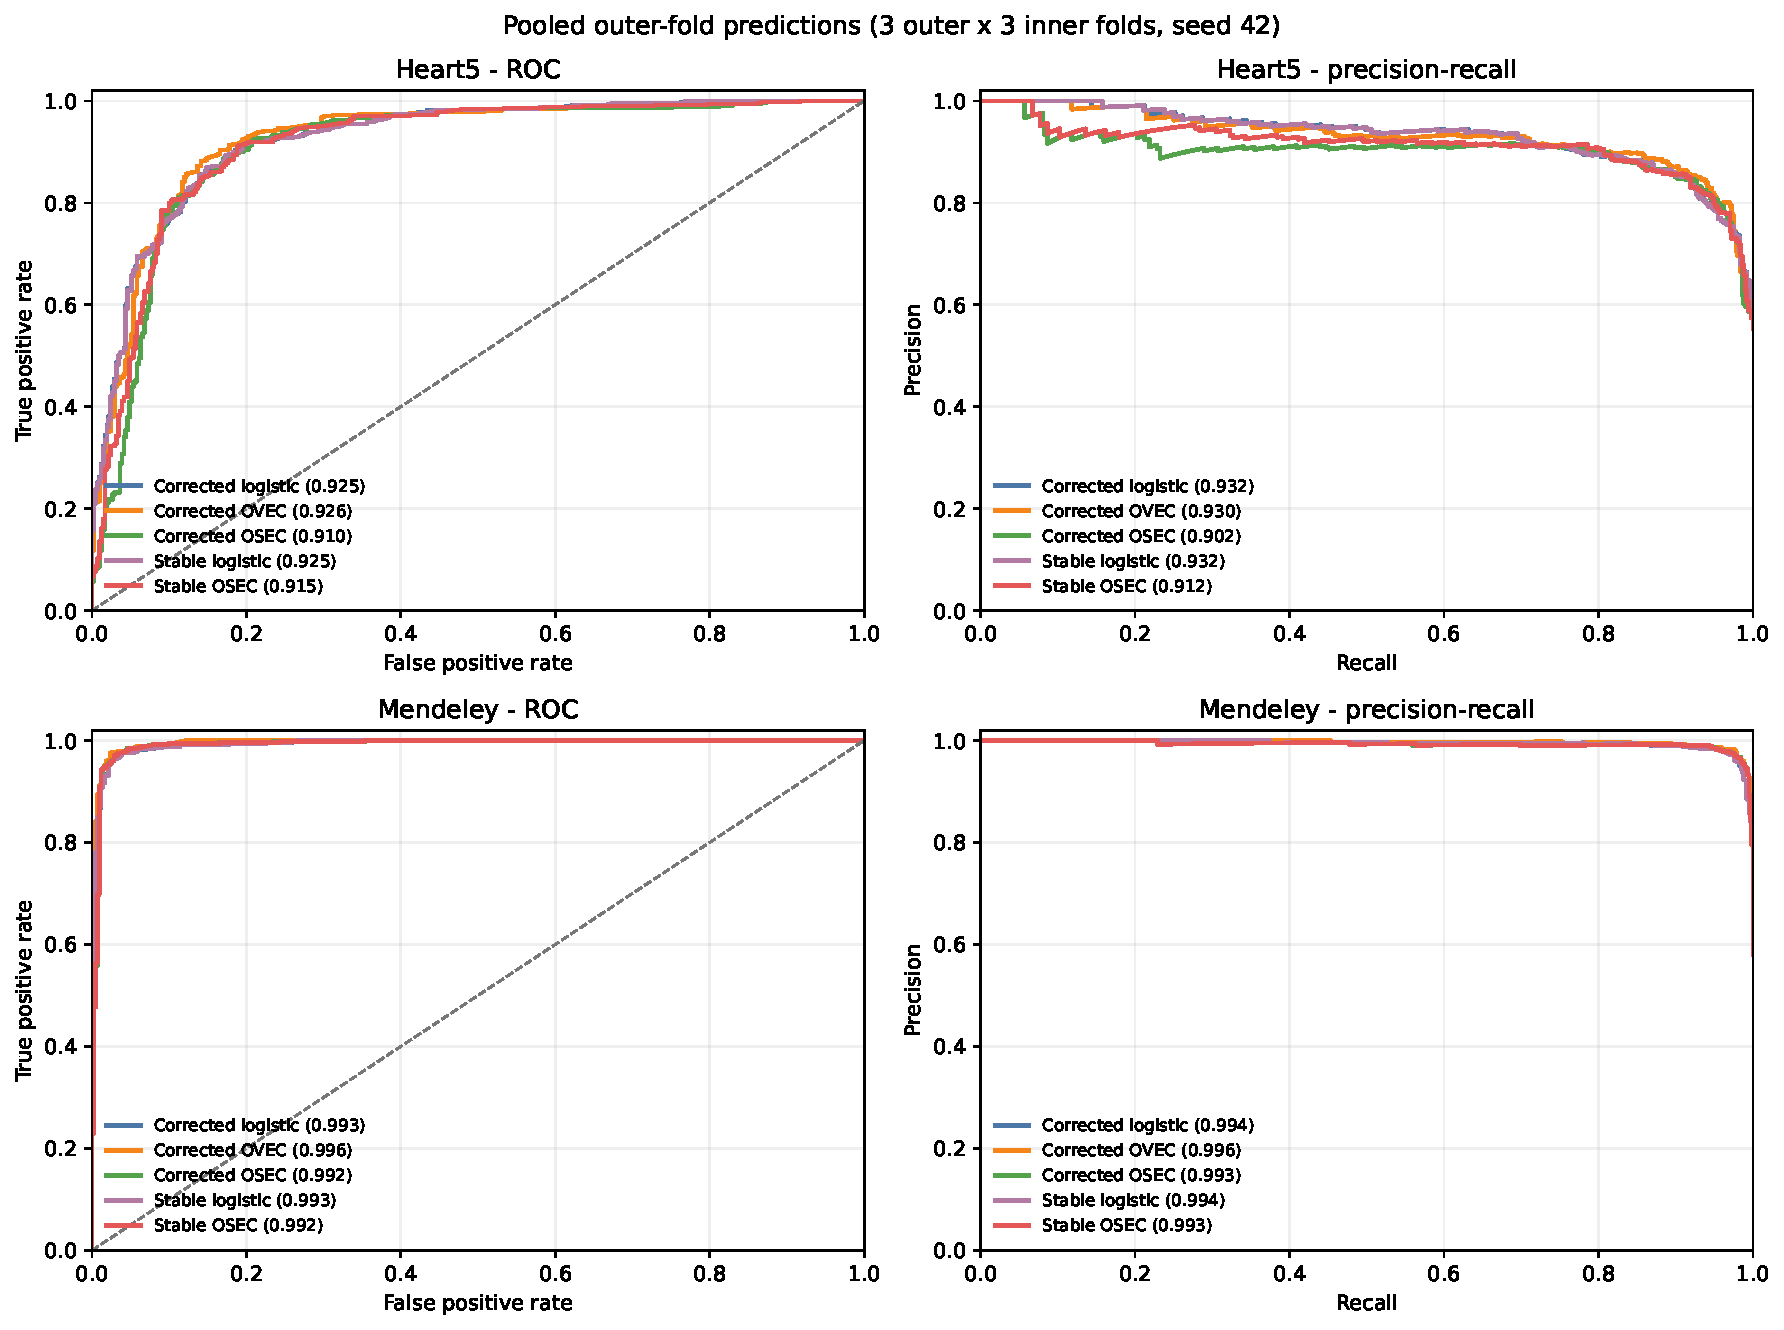
\includegraphics[width=0.98\textwidth]{figures/master_directive_20261105_final/nested_roc_pr_curves.pdf}
\caption{ROC and precision--recall curves from pooled outer-fold probabilities
for the three-outer-by-three-inner, seed-42 nested runs. Legend values are
pooled scores; the main result table reports fold means.}
\label{fig:nested-curves}
\end{figure*}

\begin{figure*}[t]
\centering
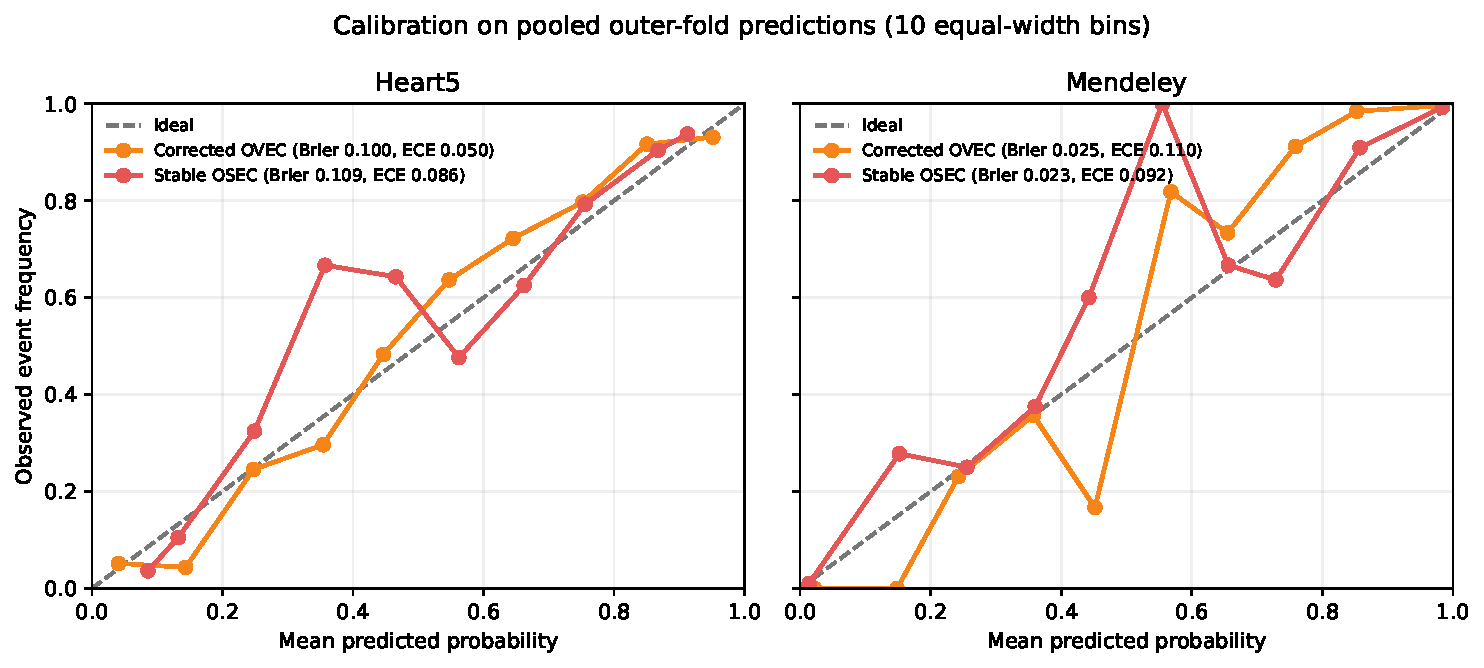
\includegraphics[width=0.88\textwidth]{figures/master_directive_20261105_final/nested_calibration.pdf}
\caption{Ten-bin calibration plots on pooled outer-fold predictions. The
Mendeley reliability curves are irregular and ECE is material despite high
discrimination, illustrating that ROC-AUC alone does not establish calibrated
probabilities.}
\label{fig:calibration}
\end{figure*}

\begin{figure*}[t]
\centering
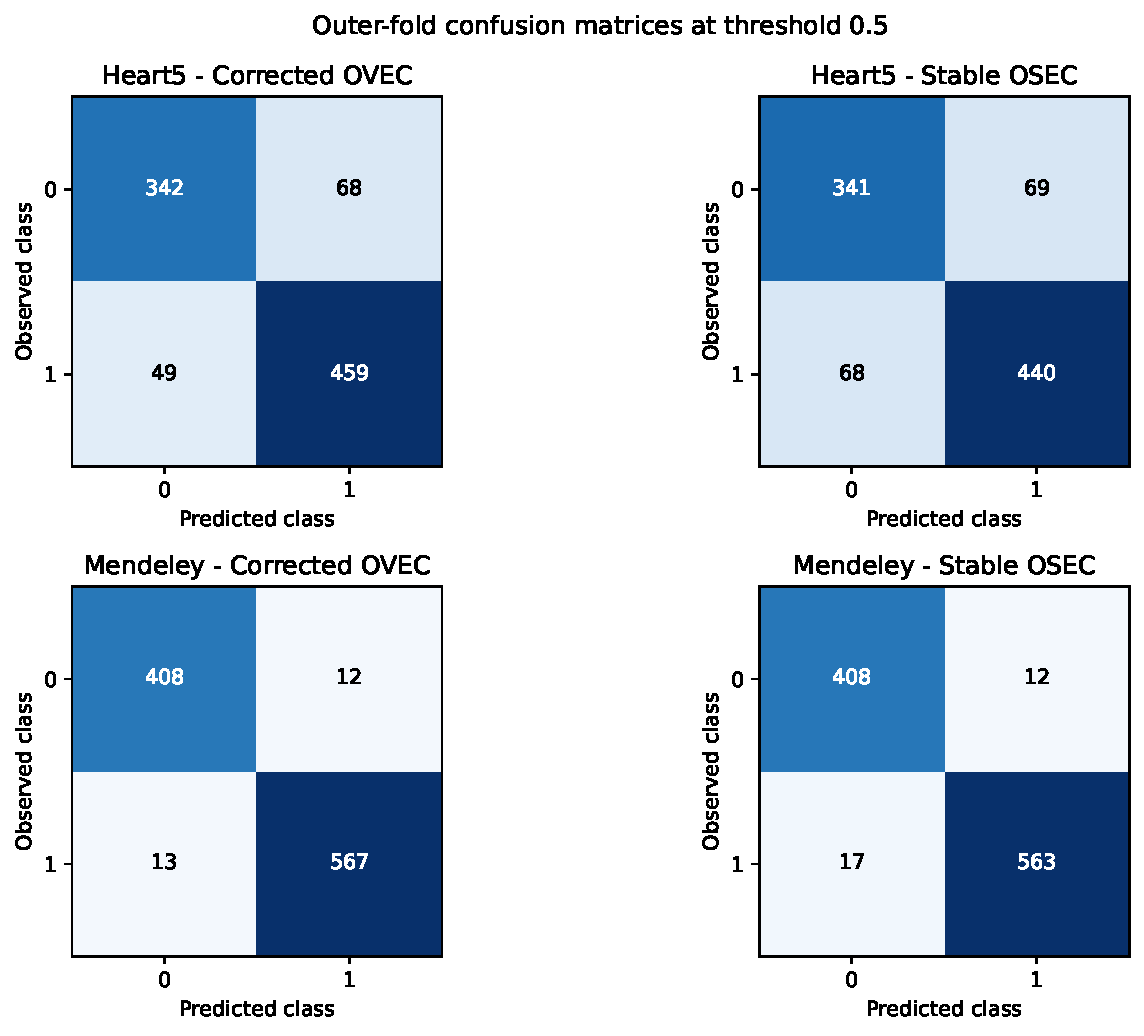
\includegraphics[width=0.82\textwidth]{figures/master_directive_20261105_final/nested_confusion_matrices.pdf}
\caption{Pooled outer-fold confusion matrices at a fixed 0.5 probability
threshold. Threshold-specific counts are descriptive and are not a substitute
for the threshold selection protocol or a clinical operating point.}
\label{fig:confusion}
\end{figure*}

\begin{figure*}[t]
\centering
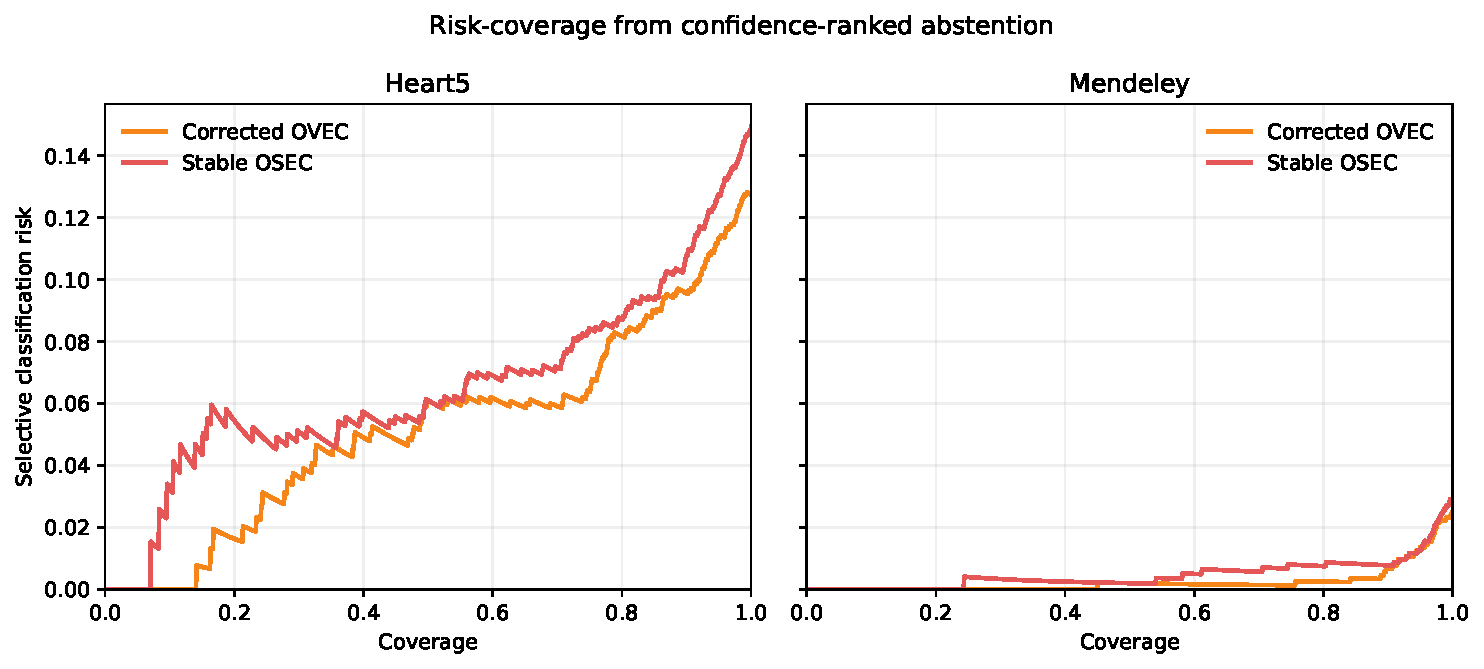
\includegraphics[width=0.88\textwidth]{figures/master_directive_20261105_final/nested_risk_coverage.pdf}
\caption{Selective classification risk as lower-confidence predictions are
abstained from. Curves describe internal pooled outer-fold predictions and do
not certify safety or clinical benefit.}
\label{fig:risk-coverage}
\end{figure*}

\begin{figure*}[t]
\centering
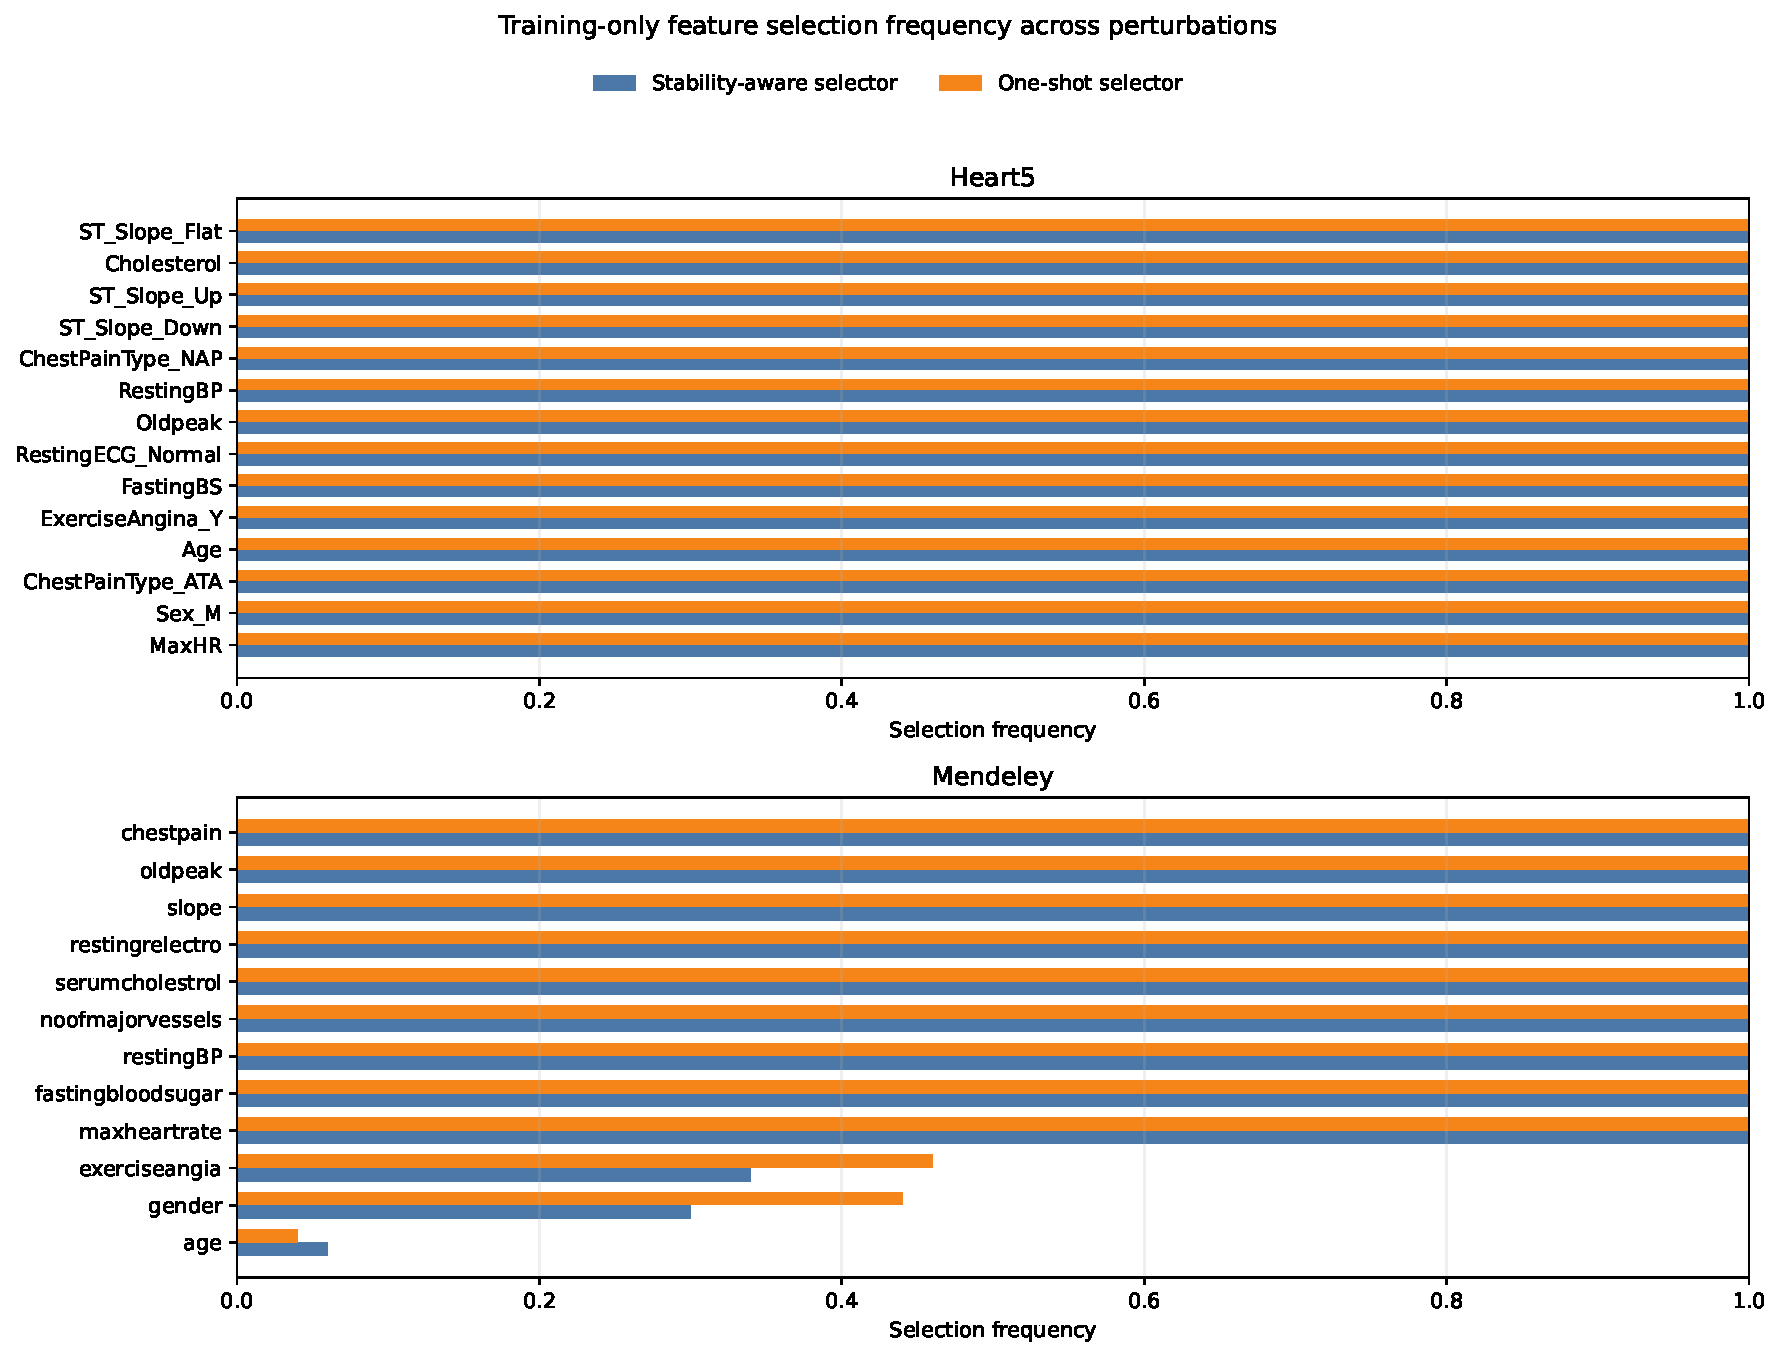
\includegraphics[width=0.98\textwidth]{figures/master_directive_20261105_final/feature_selection_stability.pdf}
\caption{Training-only feature selection frequencies under the stored
perturbation analysis. These frequencies measure feature-set stability; they
are not LIME explanation stability or evidence of causal importance.}
\label{fig:feature-stability}
\end{figure*}

\begin{figure*}[t]
\centering
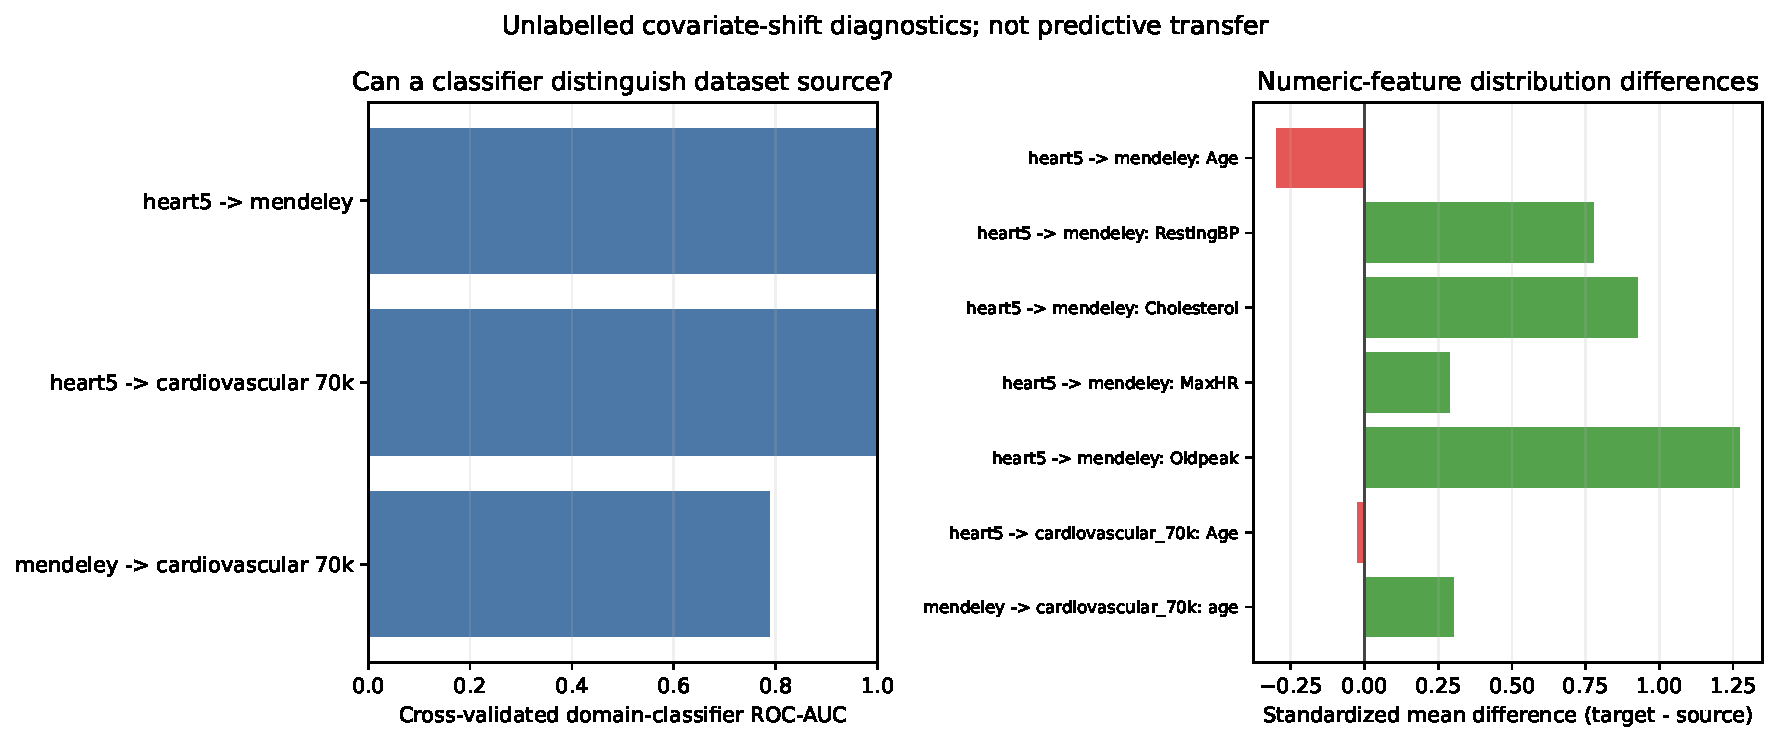
\includegraphics[width=0.98\textwidth]{figures/master_directive_20261105_final/distribution_shift_diagnostics.pdf}
\caption{Unlabelled distribution diagnostics across local datasets. Domain
classifier discrimination and standardized mean differences indicate
covariate differences only; endpoints are not semantically aligned and no
predictive transfer is evaluated.}
\label{fig:distribution-shift}
\end{figure*}

\begin{figure*}[t]
\centering
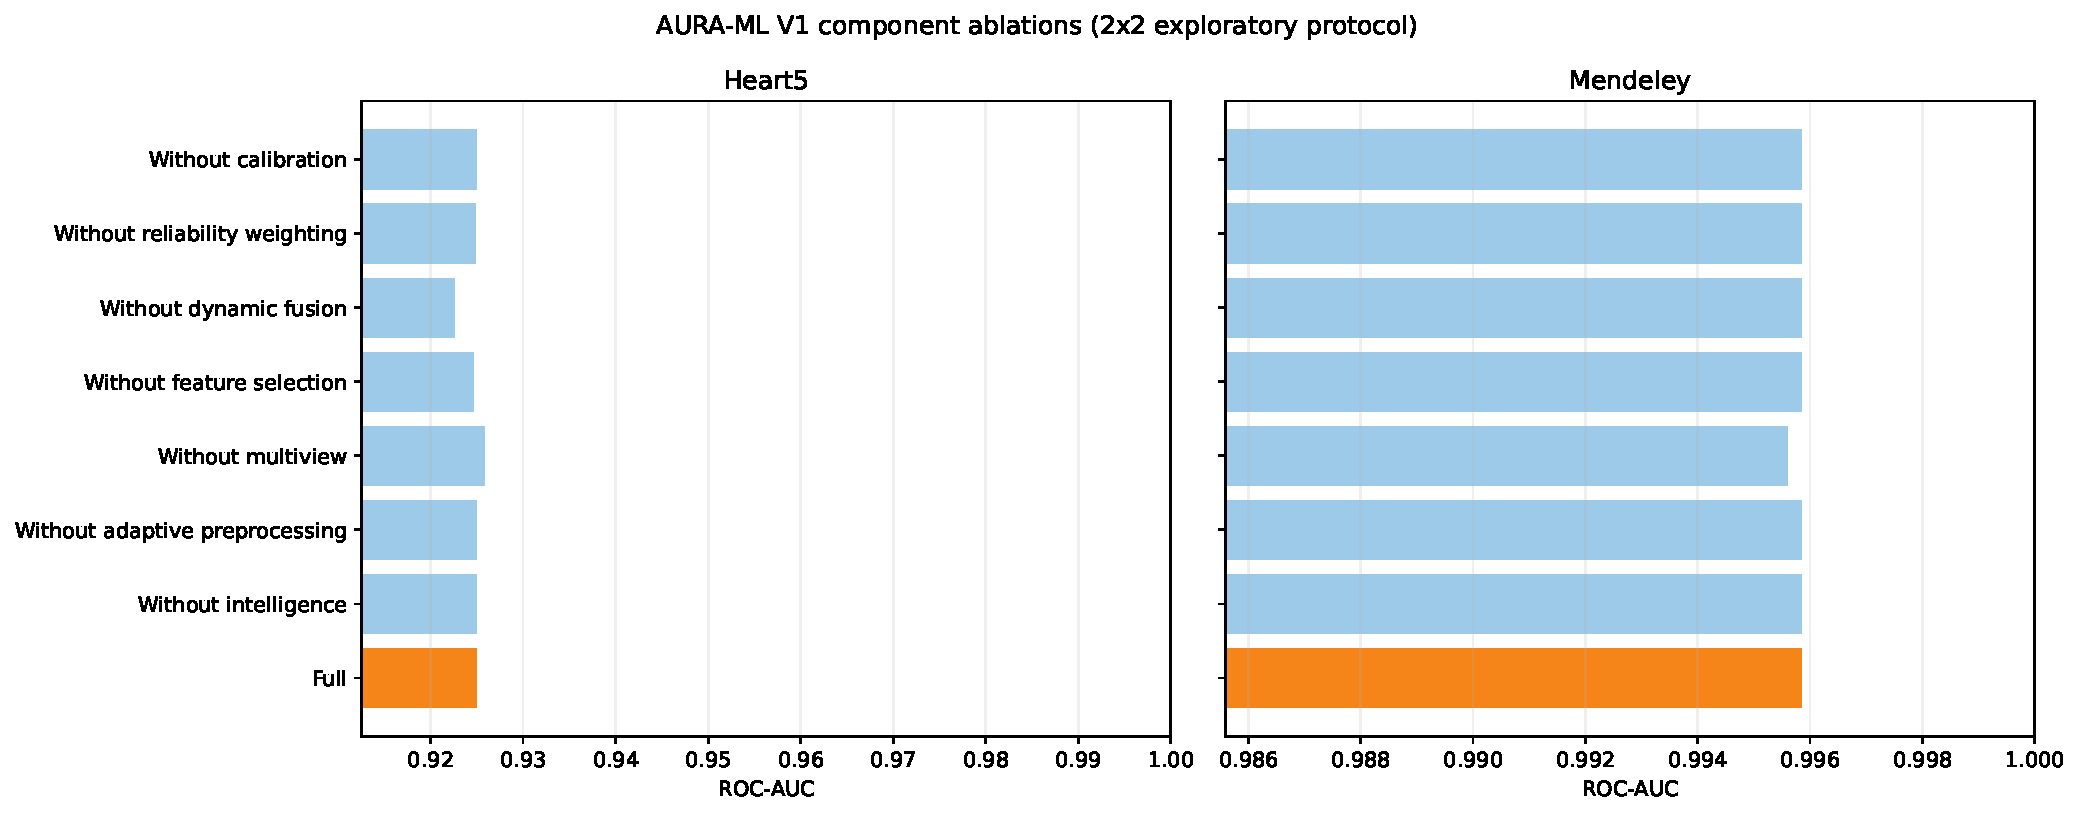
\includegraphics[width=0.98\textwidth]{figures/master_directive_20261105_final/aura_v1_ablation_roc_auc.pdf}
\caption{Exploratory AURA-ML V1 component ablations under the stored 2-by-2
protocol. These bounded results motivate a dataset-conditional interpretation
and do not establish an improved general algorithm.}
\label{fig:aura-ablation}
\end{figure*}

\begin{figure*}[t]
\centering
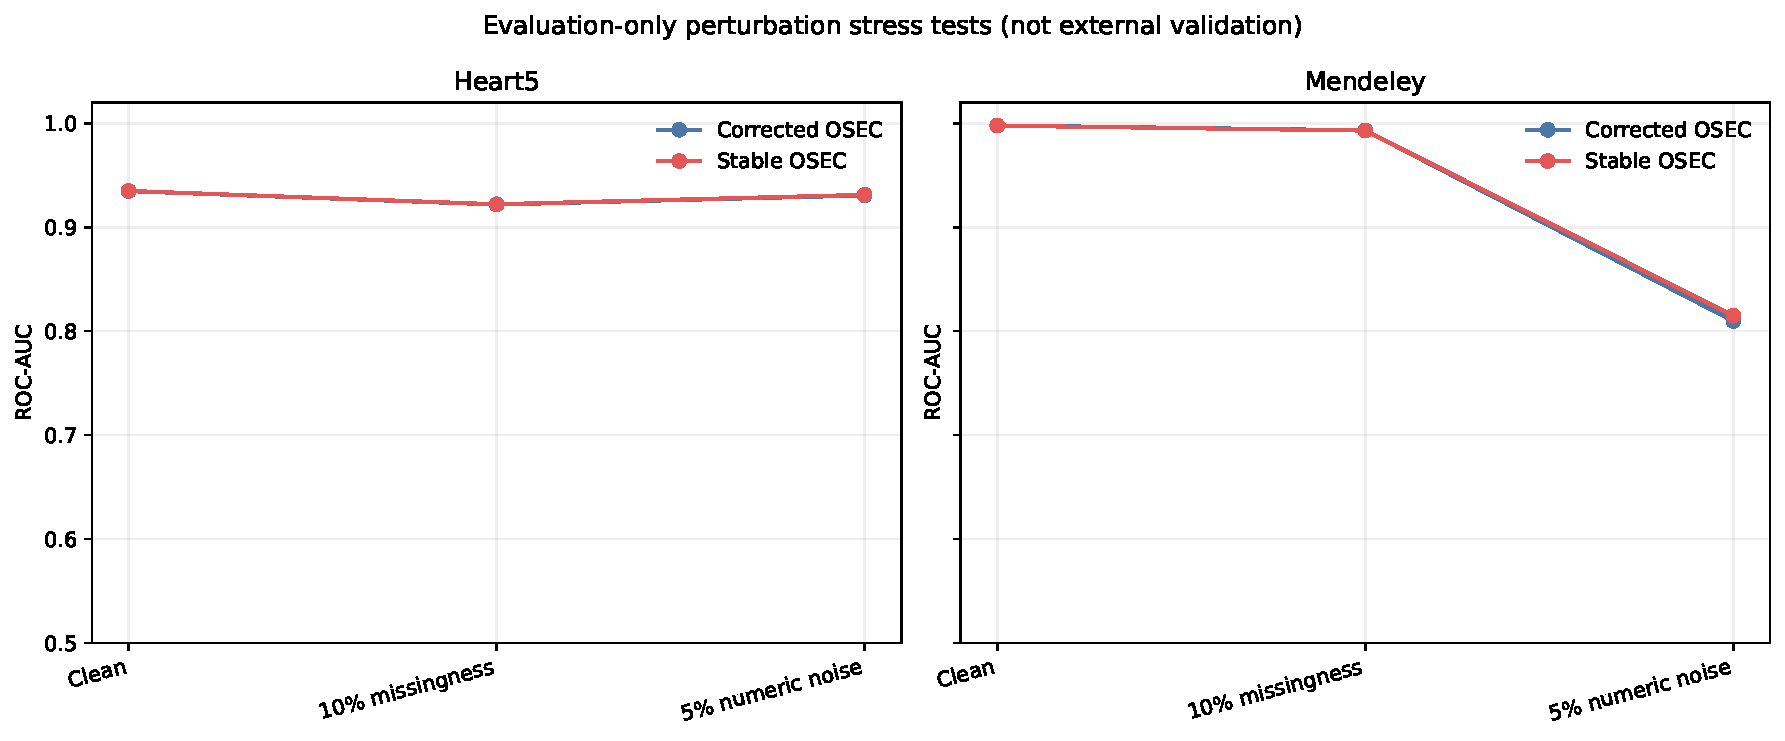
\includegraphics[width=0.98\textwidth]{figures/master_directive_20261105_final/robustness_stress_tests.pdf}
\caption{Evaluation-only synthetic missingness and numeric-noise stress tests.
The perturbations are not external data and should not be interpreted as
population transport estimates.}
\label{fig:stress-tests}
\end{figure*}

\subsection{Nested Validation}
The corrected nested runs used three outer folds, one outer repeat, and
three-fold inner selection with ROC-AUC scoring. Corrected OVEC had the
highest listed fold-mean ROC-AUC on both datasets: 0.9295 on Five States and
0.9957 on Mendeley. Stable OSEC was 0.9253 versus corrected OSEC 0.9259 on
Five States, and 0.9942 versus 0.9943 on Mendeley. The small differences do
not establish a uniform predictive advantage. Stable-candidate threshold
tuning occurred inside inner folds over 0.5, 0.75, and 1.0; these results
therefore are not numerically interchangeable with the fixed-threshold
stability experiment.

\subsection{Feature and Harmonization Sensitivity}\label{sec:validity-sensitivity}
The Mendeley nested runs were repeated with the same outer and inner splits
after excluding \texttt{noofmajorvessels}. Across the five candidates, the
fold-mean ROC-AUC changed by only +0.0003 to +0.0007
(Table~\ref{tab:mendeley-validity-sensitivity}). Thus, this one potentially
downstream variable does not explain the high internal discrimination. The
unspecified target reference
standard and the timing of the remaining predictors still prevent an
early-detection interpretation.

The AngioCAD feature sensitivity removed FBS from both source fitting and
target scoring while retaining the source partitions. This is post hoc because
AngioCAD had already been examined. In the seven-subset replay, source-Platt
ROC-AUC was 0.788 for age plus sex and 0.787 when FBS was added; the paired
candidate-minus-reference AUC difference was -0.0009 (95\% conditional
interval -0.0060 to 0.0048). Brier score and ECE were 0.176 and 0.196 for
age plus sex versus 0.185 and 0.216 for age, sex, and FBS. These comparisons
are unadjusted and do not validate the FBS unit. The AngioCAD workbook also
does not state the age unit, so age-as-years remains provisional. The separate
age/sex Isolation Forest replay had source-versus-target AUROC 0.544 (95\%
interval 0.496--0.592), consistent with no useful separation. The sensitivity
does not establish reliable shift detection
(Tables~\ref{tab:angiocad-validity-sensitivity} and
\ref{tab:angiocad-feature-ablation}).

\begin{table*}[t]
\centering
\caption{Mendeley nested-validation sensitivity after excluding the potentially
post-diagnostic fluoroscopy-derived predictor. Entries are fold-mean ROC-AUC
$\pm$ fold standard deviation across the same three outer folds; they are
descriptive, not patient-level confidence intervals.}
\label{tab:mendeley-validity-sensitivity}
\begin{tabular}{lrrr}
\toprule
Candidate & All predictors & Excluding major vessels & Difference \\
\midrule
corrected\_logistic & 0.9930 $\pm$ 0.0036 & 0.9933 $\pm$ 0.0039 & +0.0003 \\
corrected\_ovec & 0.9957 $\pm$ 0.0013 & 0.9961 $\pm$ 0.0025 & +0.0003 \\
corrected\_osec & 0.9943 $\pm$ 0.0037 & 0.9949 $\pm$ 0.0045 & +0.0007 \\
stable\_logistic & 0.9930 $\pm$ 0.0037 & 0.9933 $\pm$ 0.0039 & +0.0003 \\
stable\_osec & 0.9942 $\pm$ 0.0037 & 0.9948 $\pm$ 0.0043 & +0.0006 \\
\bottomrule
\end{tabular}

\end{table*}

\begin{table*}[t]
\centering
\caption{Post-hoc AngioCAD sensitivity to the undocumented FBS unit. Predictive
bootstrap intervals condition on the 79 negative and 298 positive matched
records. OOD intervals compare source-calibration and target feature scores.}
\label{tab:angiocad-validity-sensitivity}
\begin{tabular}{lrrrr}
\toprule
Features & Raw AUC (95\% CI) & Calibrated Brier & Calibrated ECE & OOD AUC (95\% CI) \\
\midrule
Age, sex, FBS & 0.787 (0.734--0.838) & 0.185 & 0.216 & 0.589 (0.541--0.635) \\
Age, sex only & 0.788 (0.734--0.838) & 0.176 & 0.196 & 0.544 (0.496--0.592) \\
\bottomrule
\end{tabular}

\end{table*}

\begin{table*}[t]
\centering
\caption{Post-hoc source-calibrated AngioCAD feature ablation using frozen UCI source partitions. Target-label results are descriptive, unadjusted for seven comparisons, and are not fresh validation. FBS-containing rows assume AngioCAD FBS is measured in mg/dL. Age + sex excludes FBS, but the workbook does not state age units, so age-as-years remains provisional. Intervals are class-stratified bootstrap intervals conditional on the previously examined target cohort.}
\label{tab:angiocad-feature-ablation}
\scriptsize
\begin{tabular}{lcccc}
\toprule
Features & Source-Platt ROC-AUC (95\% CI) & Brier & 10-bin ECE & Unit status \\
\midrule
Age & 0.639 (0.579--0.702) & 0.190 & 0.174 & Age-as-years assumed \\
Sex & 0.690 (0.628--0.747) & 0.194 & 0.211 & Categorical \\
Age + sex & 0.788 (0.734--0.842) & 0.176 & 0.196 & FBS excluded; age unit assumed \\
FBS & 0.354 (0.306--0.401) & 0.205 & 0.195 & mg/dL assumption \\
Age + FBS & 0.632 (0.570--0.694) & 0.199 & 0.192 & mg/dL and age-unit assumptions \\
Sex + FBS & 0.771 (0.717--0.823) & 0.202 & 0.233 & mg/dL assumption \\
Age + sex + FBS & 0.787 (0.733--0.840) & 0.185 & 0.216 & mg/dL and age-unit assumptions \\
\bottomrule
\end{tabular}
\end{table*}


\subsection{Reliability}
The linkage artifacts compare stable OSEC with corrected OSEC over ten seeds.
Confidence-error AUC was above 0.5 for both candidates on both benchmarks, but
the paired differences did not consistently favor the stable selector.
Conformal coverage was measured on the evaluation partition and is not a
guarantee under shift. The linkage intervals and rank correlations are
descriptive and exploratory.

\begin{table*}[t]
\centering
\caption{Ten-seed internal selective-reliability summaries from the
post-boundary-corrected linkage artifacts. Paired differences and descriptive
bootstrap intervals are reported in Table~\ref{tab:linkage}; these are not
independent external-validation estimates.}
\label{tab:uncertainty}
\begin{tabular}{llrrrr}
\toprule
Dataset & Candidate & Conf.-error AUC & AURC & Conformal coverage & ECE \\
\midrule
Five States & Corrected OSEC & 0.761 & 0.0505 & 0.914 & 0.121 \\
Five States & Stable OSEC & 0.760 & 0.0516 & 0.915 & 0.121 \\
Mendeley & Corrected OSEC & 0.905 & 0.0041 & 0.914 & 0.221 \\
Mendeley & Stable OSEC & 0.905 & 0.0042 & 0.914 & 0.217 \\
\bottomrule
\end{tabular}

\end{table*}

\subsection{Feature-Selection Stability}
The post-boundary-corrected stability comparison is shown in
Table~\ref{tab:stability}. The stable-minus-one-shot differences were 0.0974
(95\% descriptive bootstrap interval [-0.0272, 0.1978]) on Five States and
0.0687 ([0.0000, 0.1671]) on Mendeley. The Mendeley interval touches zero,
and the artifact's prespecified positive-evidence flag is false. These
intervals are based on only three repeat-level differences and should be
interpreted as limited comparative evidence, not patient-level confidence
intervals or proof of generality.

\begin{table*}[t]
\centering
\caption{Post-boundary-corrected feature-selection stability. $\Phi$ is the
Nogueira chance-corrected stability statistic; intervals summarize the three
repeat-level paired differences and are exploratory.}
\label{tab:stability}
\begin{tabular}{lrrrr}
\toprule
Dataset & Stable $\Phi$ & One-shot $\Phi$ & Difference & 95\% bootstrap CI \\
\midrule
Five States & 0.112 & 0.014 & 0.097 & [-0.027, 0.198] \\
Mendeley & 0.284 & 0.215 & 0.069 & [0.000, 0.167] \\
\bottomrule
\end{tabular}

\end{table*}

\subsection{Stability--Reliability Linkage}
Table~\ref{tab:linkage} tests whether a more stable selected set translated into
better held-out reliability on the same repeated splits. Differences are
stable OSEC minus corrected OSEC; positive AURC or ECE differences indicate
worse selective risk or calibration, respectively. The paired intervals include
zero for all listed comparisons. On Mendeley, ROC-AUC, AURC, and
full-coverage risk favored corrected OSEC, while the other intervals included
zero. Thus, selector stability did not act as a consistent surrogate for
predictive or selective reliability.

\begin{table*}[t]
\centering
\caption{Paired stability--reliability linkage. $\Phi$ is cross-seed selected-
set stability. $\Delta$ values are stable OSEC minus corrected OSEC means; the
full bootstrap intervals are stored in the machine-readable linkage artifacts.}
\label{tab:linkage}
\begin{tabular}{lrrrrr}
\toprule
Dataset & Cross-seed $\Phi$ & $\Delta$ ROC-AUC & $\Delta$ Conf.-AUC & $\Delta$ AURC & $\Delta$ ECE \\
\midrule
Five States & 0.201 & -0.0009 & -0.0015 & +0.0011 & -0.0001 \\
Mendeley & 0.178 & -0.0002 & -0.0001 & +0.0002 & -0.0045 \\
\bottomrule
\end{tabular}

\end{table*}

\subsection{Z-Alizadeh Sani Site-Level Stress Test}
After the source-only protocol was frozen, a single model was trained on all
four UCI source cohorts and evaluated once on the separately reported
Z-Alizadeh Sani cohort. The harmonized inputs were age, sex, and
fasting-glucose status;
the predictor was fixed logistic regression, with equal total fitting weight
per source cohort. A Platt calibrator and Isolation Forest warning threshold
were fit using source data only. The external cohort had 303 records, including
216 CAD and 87 Normal labels. No target labels were used for fitting,
calibration, or threshold selection.

The source-only model achieved ROC-AUC 0.720 (class-stratified bootstrap 95\%
CI 0.651--0.780) and average precision 0.853 (0.807--0.894). Platt calibration
reduced Brier score from 0.200 to 0.193 and 10-bin ECE from 0.136 to 0.110;
paired bootstrap intervals for these differences included zero. The OOD score
separated source calibration and target rows weakly (AUROC 0.604, 95\% CI
0.552--0.652) and flagged 14.9\% of target rows at a 5.3\% source calibration
false-alert rate. Flagged rows had a Brier score of 0.238, versus 0.185 in
accepted rows, but only five flagged rows were negative. The result does not
establish reliable rejection or calibration under shift.

The target site's outcome uses \(\geq 50\%\) stenosis, while the source
outcome uses \(>50\%\); individual stenosis values are unavailable to
reconcile the cut point. The public files also have no patient identifiers for
record-level overlap checks. We therefore describe this as a site-level
transport stress test, not verified patient-independent or endpoint-identical
external validation. The
measured cohort is small and single-site, and does not estimate variation
across hospitals or time.

\begin{table*}[t]
\centering
\caption{Source-only transfer results on the Z-Alizadeh Sani cohort. Bootstrap
intervals condition on the observed target class counts.}
\label{tab:zas-transfer}
\begin{tabular}{lcc}
\toprule
Metric & Estimate & 95\% interval \\
\midrule
ROC-AUC & 0.720 & 0.651--0.780 \\
Average precision & 0.853 & 0.807--0.894 \\
Brier, raw / calibrated & 0.200 / 0.193 & 0.192--0.208 / 0.174--0.213 \\
ECE, raw / calibrated & 0.136 / 0.110 & 0.115--0.172 / 0.097--0.154 \\
OOD AUROC & 0.604 & 0.552--0.652 \\
\bottomrule
\end{tabular}
\end{table*}

\begin{figure*}[t]
\centering
\includegraphics[width=\textwidth]{../results/transfer_20261105_zas_external/external_transfer_summary.png}
\caption{Source-only transfer results for the Z-Alizadeh Sani cohort. The
calibration and OOD components were fit using source data only. The outcome
boundary differs at exactly 50\% stenosis, so this is a transport stress test.}
\label{fig:zas-transfer}
\end{figure*}

\subsection{Endpoint-Aligned AngioCAD Site Evaluation (Post Hoc)}
The frozen \texttt{CD-XD-004} pipeline evaluated AngioCAD after source-only
fitting and threshold selection. The analysis used 377 matched records from
the reported Isfahan hospital, of which 298 (79.0\%) were positive and 79 were
negative. The dataset article reports 413 patients, but the released clinical
feature workbook lacks rows for 36 labeled IDs. Age and FBS were missing for 6
and 11 matched patients, respectively, and were imputed using source-fit
values. The target was positive when any of 15 artery segments had a stenosis
category above 50\%; this aligns the UCI source endpoint. No cross-dataset
person-level linkage was possible.

The source-only predictor achieved ROC-AUC 0.787 (class-stratified bootstrap
95\% CI 0.734--0.838) and average precision 0.932 (0.913--0.952). Platt
calibration did not change ranking. It reduced Brier score from 0.190 to 0.185
and log loss from 0.569 to 0.548 by point estimate, while 10-bin ECE increased
from 0.211 to 0.216. Paired bootstrap intervals for the Brier-score change
(-0.0133 to 0.0049), log-loss change (-0.0415 to 0.0006), and ECE change
(-0.0213 to 0.0164) included no difference. Mean predicted risk after
calibration was 0.574, below the observed 0.790 positive fraction; the
calibration intercept and slope were 1.219 and 1.436. Thus the small Brier and
log-loss improvements do not establish adequate target calibration.

The OOD detector flagged 44/377 (11.7\%) target records, with 88.3\% accepted
coverage and a 5.3\% source-calibration false-alert rate. Source-versus-target
OOD AUROC was 0.589 (95\% CI 0.541--0.635), indicating weak separation. The
calibrated Brier score was 0.179 among accepted records and 0.233 among the 44
flagged records. This descriptive difference is not evidence that the warning
reliably identifies individual errors.

\begin{table*}[t]
\centering
\caption{Source-only transfer results on the endpoint-aligned AngioCAD cohort.
Bootstrap intervals condition on the 79 negative and 298 positive matched
records.}
\label{tab:angiocad-transfer}
\begin{tabular}{lcc}
\toprule
Metric & Raw & Source Platt calibrated \\
\midrule
ROC-AUC & 0.787 (0.734--0.838) & 0.787 (0.734--0.838) \\
Average precision & 0.932 (0.913--0.952) & 0.932 (0.913--0.952) \\
Brier score & 0.190 (0.184--0.196) & 0.185 (0.171--0.200) \\
Log loss & 0.569 (0.556--0.581) & 0.548 (0.516--0.580) \\
10-bin ECE & 0.211 (0.203--0.232) & 0.216 (0.198--0.234) \\
Balanced accuracy at 0.5 & 0.630 & 0.719 \\
Sensitivity at 0.5 & 0.906 & 0.728 \\
Specificity at 0.5 & 0.354 & 0.709 \\
\bottomrule
\end{tabular}
\end{table*}

\subsection{Source-Domain Abstention and Operating Boundary}
CD-XD-006 re-ran the endpoint-aligned AngioCAD transfer with disjoint
probability and conformal-calibration partitions. The source-only predictor
achieved ROC-AUC 0.790 (95\% class-stratified bootstrap CI 0.733--0.837).
Platt calibration changed Brier score from 0.189 to 0.174 and 10-bin ECE from
0.211 to 0.192. The 90\% source-domain conformal set covered all 377 target
records empirically, but only 33 (8.8\%) received singleton sets. After
combining singleton-set and feature-support rules, only 21 (5.6\%) received
automatic outputs; no errors were observed, but all 21 accepted records were
positive. This small one-class subset does not establish low error at a useful
operating coverage. The kNN feature
support detector separated target from source calibration rows weakly
(AUROC 0.580, 95\% CI 0.527--0.635).

The metadata-based operating-domain gate withheld probabilities for all 377
AngioCAD records because the site is not in the UCI source registry. This gate
is deterministic when trusted site metadata is provided; it is not a
feature-based estimate of domain membership. CD-XD-006 is a post-hoc policy
replay because AngioCAD outcomes had already been examined in CD-XD-004.

CD-XD-005 evaluated the same abstention method on the newly sourced Duke
cohort, using age, sex, and cholesterol. ROC-AUC was 0.661 (95\% bootstrap CI
0.642--0.680). Source Platt calibration worsened Brier score from 0.216 to
0.241 and ECE from 0.119 to 0.198. The kNN and Isolation Forest OOD AUROCs
were 0.556 and 0.598, respectively. The conformal set covered 98.3\% of Duke
records empirically but was singleton for 13.9\%; the combined method
automatically classified 401 (11.4\%) with 41 errors (10.2\%). The site gate
withheld probabilities for all 3,504 records. Because Duke's endpoint begins
at 75\% stenosis, these differences combine cohort, endpoint, and measurement
shift and are not a direct test of same-endpoint generalization.

An independent post-hoc component audit recalculated coverage and accepted
errors for the frozen probability, conformal, kNN, Isolation Forest, combined,
and site-gate policies. The detector-only rules retain 93.4--99.7\% coverage
on AngioCAD while leaving the fixed-threshold error rate essentially
unchanged. The registered conformal+kNN combination covers only 5.6\% on
AngioCAD and 11.4\% on Duke. The unknown-site registry gate remains at 0\%
coverage for both cohorts. Component results are descriptive and did not
select the deployed policy (Table~\ref{tab:selective-policy-components}).

\begin{table*}[t]
\centering
\caption{Post-hoc comparison of frozen selective-policy components. AngioCAD was previously examined; Duke uses a different endpoint. The registry blocks both unregistered cohorts. Target labels did not select thresholds or policies.}
\label{tab:selective-policy-components}
\scriptsize
\begin{tabular}{lrrrr}
\toprule
Policy & AngioCAD coverage & AngioCAD errors & Duke coverage & Duke errors \\
\midrule
Fixed probability 0.5, no abstention & 100.0\% & 96/377 & 100.0\% & 1,358/3,504 \\
Conformal singleton only & 8.8\% & 0/33 (0.0\%) & 13.9\% & 61/487 (12.5\%) \\
kNN detector only & 93.4\% & 93/352 (26.4\%) & 95.6\% & 1,305/3,349 (39.0\%) \\
Isolation Forest only & 99.7\% & 96/376 (25.5\%) & 97.3\% & 1,330/3,409 (39.0\%) \\
Registered conformal + kNN & 5.6\% & 0/21 (0.0\%); one class & 11.4\% & 41/401 (10.2\%) \\
Unknown-site registry gate & 0.0\% & No score emitted & 0.0\% & No score emitted \\
\bottomrule
\end{tabular}
\end{table*}


\begin{table*}[t]
\centering
\caption{Source-only transfer and abstention results. AngioCAD was previously examined; Duke uses a different stenosis threshold. The registry gate withholds scores for both unregistered target sites.}
\label{tab:domain-guard-transfer}
\begin{tabular}{lcc}
\toprule
Metric & AngioCAD ($n=377$) & Duke ACATH ($n=3{,}504$) \\
\midrule
Endpoint & >50\% aligned & $\geq$75\% mismatch \\
ROC-AUC (95\% bootstrap CI) & 0.790 (0.733--0.837) & 0.661 (0.642--0.680) \\
Brier score (raw / Platt) & 0.189 / 0.174 & 0.216 / 0.241 \\
10-bin ECE (raw / Platt) & 0.211 / 0.192 & 0.119 / 0.198 \\
90\% conformal set coverage & 100.0\% & 98.3\% \\
Singleton-set coverage & 8.8\% & 13.9\% \\
Combined automatic coverage & 5.6\% & 11.4\% \\
Errors among automatic outputs & 0/21 & 41/401 (10.2\%) \\
OOD AUROC (kNN / IF) & 0.580 / 0.579 & 0.556 / 0.598 \\
Registry-gate automatic coverage & 0.0\% & 0.0\% \\
\bottomrule
\end{tabular}
\end{table*}


\begin{figure*}[t]
\centering
\includegraphics[width=0.96\textwidth]{../results/transfer_20261105_angiocad_domain_guard/figures/angiocad_transport_reliability.png}
\caption{CD-XD-006 post-hoc AngioCAD replay. The source-calibrated model's
feature-support distributions overlap, and confidence ranking does not remove
the need for the source-domain gate. All AngioCAD rows are withheld by that
gate because the target site is unregistered.}
\label{fig:angiocad-domain-guard}
\end{figure*}

\subsection{External Cohort Evaluation and Threats to Validity}
The Z-Alizadeh Sani run is from a separately reported hospital, but
its threshold includes exactly 50\% stenosis and participant-level overlap
cannot be checked; it remains a transport stress test. AngioCAD is one
separately reported site with an endpoint-near target, but only 377 of 413
labeled IDs had feature rows, common person identifiers are unavailable, and
the target had already been examined. The supplied Mendeley dataset was used
in the base paper; the public UCI component sources overlap the Five States
composite. Thus, the available evidence does not establish verified
patient-independent external validation. The AngioCAD results show moderate
ranking but weak calibration and weak feature-only OOD separation. The site
gate withholds scores for unregistered cohorts; 0\% automatic coverage on both
evaluated target sites is not a useful operating point. Duke ACATH is a
reported separate-site stress test, but its \(\geq75\%\) endpoint differs from
UCI's \(>50\%\) endpoint and participant linkage is unavailable. Additional
endpoint-compatible hospitals and temporal or prospective evaluation remain
necessary before making broad generalization claims. This caution is
consistent with documented
heterogeneity and performance degradation when cardiovascular prediction
models are evaluated outside their development data
\cite{wessler2021external}.

\subsection{Statistical Analysis and Robustness}
The study prespecifies ROC-AUC as the primary comparison and reports PR-AUC,
classification metrics, Brier score, calibration intercept and slope, uniform
ten-bin ECE, selected-set stability, confidence-error AUC, AURC, and conformal
coverage as secondary quantities. Paired comparisons use identical partitions
for the candidates. No multiplicity-adjusted confirmatory claim is made across
the secondary metrics. Synthetic missingness or measurement perturbations,
when run, will be reported as stress tests and not as independent validation.

The post-boundary-corrected stability runs found differences of 0.0974
[-0.0272, 0.1978] on Five States and 0.0687 [0.0000, 0.1671] on Mendeley.
The ten-seed linkage runs found no consistent reliability advantage: the paired
ROC-AUC difference was -0.0009 [-0.0027, 0.0007] on Five States and -0.0002
[-0.0004, -0.0001] on Mendeley, while calibration and selective metrics did
not uniformly favor the stable candidate. These are bounded internal results
and remain subject to dependence, small effective replication counts, and
multiple comparisons.

The separate Kaggle benchmark produced pooled outer ROC-AUC values of 0.80043
for CatBoost and 0.80022 for XGBoost in the tuned run. The prior XGBoost
benchmark was 0.80038. The fixed uniform ensemble achieved 0.79897 and
therefore did not improve the standalone boosted models. The CatBoost
difference is marginal, exploratory, and not evidence of practical or
statistical superiority.

A compact candidate-pool rerun evaluated Elastic Net, RBF SVM, KNN, Extra
Trees, Gaussian NB, and LDA alongside the scalable boosting candidates. On
70,000 rows, RBF SVM and KNN were prespecified as computationally infeasible
and were not run. In that separate protocol, stacking achieved pooled
ROC-AUC 0.80028, XGBoost 0.80008, CatBoost 0.79998, and fixed soft voting
0.79943. The small differences do not establish an ensemble or model
superiority.

An evaluation-only stress test at seed 42 applied 10\% independent missingness
and numeric noise with standard deviation equal to 5\% of each training feature
standard deviation. On Mendeley, ROC-AUC fell from 0.998 to 0.810 under the
numeric-noise perturbation for corrected OSEC and from 0.998 to 0.815 for stable
OSEC. On Five States, 10\% missingness reduced ROC-AUC from approximately 0.935
to 0.922 for both candidates. These are synthetic single-split stress tests,
not independent external validation.

\section{Discussion}
The nested results do not support a uniform performance advantage for the
stability-aware selector. On the Five States benchmark, corrected OVEC has the
highest mean ROC-AUC among the listed candidates, while stable OSEC is lower.
On the Mendeley benchmark, corrected OVEC and stable OSEC are similar. The
post-boundary-corrected stability comparison does not establish a positive
stability advantage: its Five States interval crosses zero and its Mendeley
interval touches zero. The ten-seed reliability results do not show
consistent improvement across discrimination, selective risk, coverage, and
calibration. These findings separate feature-set stability from predictive
reliability: more repeatable feature selection does not by itself establish
better calibrated or safer predictions. A selector is not justified merely
because it reduces dimensionality or includes an explainability component.

The transport evidence is mixed. The post-hoc AngioCAD replay ranked patients
reasonably well, but automatic coverage was only 5.6\%; the feature-support
detector was weak, and the registry gate withheld every target score. The
fresh Duke cohort showed lower ranking performance, worse calibration after
source-only Platt scaling, and a 10.2\% error rate among the small subset
automatically classified. Its stricter stenosis endpoint prevents attributing
that result to dataset shift alone. Together, these results demonstrate a
working fail-closed prototype and expose its present operating boundary; they
do not establish useful predictive coverage on unseen hospitals.

\section{Limitations and Ethical Considerations}
This is a retrospective engineering evaluation using public benchmarks; it
does not estimate prospective clinical performance. Dataset provenance,
license conditions, outcome definitions, prediction timing, and possible source
overlap constrain interpretation and transportability. In particular, the
Mendeley endpoint has no documented diagnostic reference standard, and the
AngioCAD unit sensitivity is post hoc. The study does not establish broad
generalization or reliable feature-only shift recognition. The full
five-candidate custom nested protocol was not
completed on the 70,000-row Kaggle task because of computational cost; a
reduced corrected-logistic versus stable-logistic analysis is labeled
separately. The source-domain gate relies on trusted site metadata and
withheld all target predictions; the feature-only OOD score did not reliably
identify either unseen cohort. The conformal sets were calibrated on source
partitions, and external empirical coverage does not imply a distribution-free
guarantee under dataset shift.

\section{Reproducibility}
The code, tests, dependency lock, data manifests, protocol reports, and result
generators are maintained in the repository. Raw restricted data must not be
committed.

\section{Conclusion}
An exploratory AURA-ML V2 extension was subsequently evaluated under three
outer and three inner folds on seeds 42--44 for the two development benchmarks.
The V2 policy removed feature selection after its ablation evidence failed to
show a consistent benefit, and compared training-side sigmoid and isotonic
calibration and threshold selection. Seed-aggregated ROC-AUC was 0.9244 for
AURA-ML V2 versus 0.9257 for corrected OVEC on Five States, and 0.9977 versus
0.9955 on Mendeley. These results are supplementary exploratory evidence, not
external validation: the 70,000-row V2 3-by-3 attempt exceeded the local
runtime budget without producing a valid artifact, and the Mendeley benchmark
was already used in the base study.

This work delivers a reproducible leakage-controlled audit and a falsifiable
stability--reliability decoupling audit for CARDIODIAG. Internal evidence shows
that feature-set stability and selective reliability can move independently:
the corrected stability comparison does not establish a stable-selector
advantage, and the stable selector does not produce a consistent predictive or
reliability benefit.
The endpoint-aligned AngioCAD studies achieved ROC-AUC 0.787 and 0.790, but
the latter is a post-hoc replay on a previously examined target. Disjoint
source calibration modestly improved point estimates for Brier score and ECE
on AngioCAD, while conformal and feature-support rules automatically covered
only 5.6\% of its rows. The new registry gate withheld all predictions on
unregistered target sites, including AngioCAD and Duke. The Duke stress test
had a different outcome threshold and source-only Platt calibration worsened
its Brier score. Feature-only OOD separation remained weak. These findings
support a reproducible fail-closed research prototype and document its low
utility and dataset limitations; they do not establish dependable
generalization, clinical readiness, or a novel prediction algorithm.
For the stated objective of dependable, uncertainty-calibrated prediction on
unseen datasets, this is a research no-go: the available evidence fails the
claim. The engineering prototype is complete as a reproducible negative result;
reversing this decision requires untouched, endpoint-compatible external data.

\section*{Author and Publication Declarations}
\textbf{Ethics and data use:} Not determined. This study analyzes secondary
public datasets. The project team must verify dataset access and reuse terms
and obtain an institutional determination of whether ethics review or an
exemption is required. No approval or exemption is claimed in this draft.

\textbf{Funding:} Not determined; confirmation from all authors is pending.

\textbf{Author contributions:} Akhil Preetham E (provisional):
conceptualization, methodology, software development, data curation, formal
analysis, experimentation, validation, visualization, and initial manuscript
preparation. Contributions from Ch Hari Krishna and G Vennela are pending.

\textbf{Competing interests:} Not determined; all authors must disclose any
relevant interests before submission.

\textbf{Data availability:} Dataset sources, DOIs/versions, hashes, access
conditions, license findings, and attribution are recorded in the final
dataset attribution register and project manifests. No raw datasets are
included in the proposed data-free code release. The Five States composite's exact upstream record and standalone
terms are unresolved; the Kaggle 70,000-record source lists its license as
unknown; Duke redistribution terms are unspecified. These files and their
row-level derivatives are excluded from the public release manifest. The
Mendeley, UCI, Z-Alizadeh Sani and AngioCAD sources declare CC BY 4.0 and have
dataset-specific attribution notices, but their raw files are also omitted
from the proposed data-free release. Legacy ZIP archives are not approved for
public upload.

\textbf{Code availability:} The source is maintained in the project
repository. No public package has been generated or authorized. A root project
code license is absent, so redistribution authority must be confirmed before
release. Existing \texttt{dist/*.zip} snapshots are legacy artifacts and are
not approved for release; the data-free allow-list and exclusions are recorded
in the final data release manifest.

\textbf{Publication venue:} Provisional target: BMJ Health \& Care Informatics. Venue approval by all authors and final journal-specific proofing are pending.

\bibliographystyle{unsrt}
\bibliography{references}
\end{document}



